% =====================================================================================================
% Draft: three baselines for the evaluation (Section 13): vertical full-record SSP, the Ferrando--Wang--Sheldon
% parametric-bootstrap intervals, and TukeyEM.
%
% How to merge into paper/main.tex (mechanical): each block runs from "%B-BEGIN <id>" to "%B-END <id>".
%   "%AFTER| <anchor>": insert the lines between %NEW-BEGIN and %NEW-END after the line of main.tex that contains
%   the anchor (it occurs exactly once), preceded by an empty line.
%   "%OLD| <text>": replace that exact text (it occurs exactly once) by the new text.
%       python experiments/baselines/apply_baselines_draft.py --check
%       python experiments/baselines/apply_baselines_draft.py --out /tmp/main_baselines.tex
%   The script never writes main.tex. Anchors are as of commit f6ef86a (P2 and related work merged).
%   Blocks: B00 abstract sentence; B01 contributions item; B02 new subsection "Interval methods" after 13.3 (FWS);
%   B03 pointer at the end of the 13.7 setup; B04 new subsection "Two further baselines" after 13.7 (full-record SSP
%   and TukeyEM, with Proposition prop:sens_full); B05 paragraph in 13.9; B06 narrower columns in Table tab:settings
%   (the two new subsections renumber 13.4-13.9 to 13.5-13.11, and its row "used in" would overflow by 9.5pt).
%   New labels: sec:eval:fws, tab:fws_cov, fig:fws_cov, tab:fws_real, sec:eval:baselines, prop:sens_full,
%   eq:sens_full, tab:full_sim, fig:full_sim, tab:full_verdicts, fig:full_real, tab:tukey, fig:tukey.
%   New figures: paper/figures/{fws_coverage,fullrecord_sim,fullrecord_real,tukey}_base.png. Five new \tocheck items.
%   Checked: spliced into a copy of main.tex (f6ef86a), two pdflatex runs, no errors, no undefined references, no
%   overfull boxes.
%
% Sources: reports/baselines/README.md and key_numbers.md (generated by experiments/baselines/tables_base.py).
% =====================================================================================================

%B-BEGIN B00 Abstract: one sentence on the three further baselines (before the sentence on the end-to-end runs)
%OLD| with joint normalization). End-to-end runs of a full OpenFHE implementation
%NEW-BEGIN
with joint normalization). Against three further baselines, noising $\Rp$'s own block as well (full-record SSP) raises test error by a median of about $1\%$ on the 29 datasets; TukeyEM, which needs no bounds, fails its stability test and releases nothing on 25 of them at $\varepsilon \le 2$; and the parametric bootstrap of Ferrando et al., applied to our release, gives the same interval for the coefficients as ours once the ridge is off, and a finite one that covers, where ours is unbounded, from about a quarter of the ridge threshold on the synthetic population. End-to-end runs of a full OpenFHE implementation
%NEW-END
%B-END B00

%B-BEGIN B01 Contributions, evaluation item: the new baselines
%OLD| and a benchmark against AdaSSP on 29 UCI datasets, under two named settings
%NEW-BEGIN
benchmarks against AdaSSP, vertical full-record SSP and TukeyEM on 29 UCI datasets, and a comparison with the parametric-bootstrap intervals of Ferrando et al., under two named settings
%NEW-END
%B-END B01

%B-BEGIN B02 New subsection after Section 13.3 (coverage): the FWS intervals (baseline 2)
%AFTER| repeat the check on real data.}
%NEW-BEGIN
\subsection{Interval methods: the parametric bootstrap of Ferrando, Wang and Sheldon}
\label{sec:eval:fws}

Our Wald interval borrows the parametric bootstrap of Ferrando, Wang and Sheldon~\cite{ferrando2022parametric} (FWS). Their interval for differentially private least squares is also a competitor to our interval for $\bbeta$. This subsection runs it on the releases of setting I and compares coverage and width, estimand by estimand.

\paragraph{The FWS interval.} From released statistics $\hat\bG$, $\hat\bc$ and $\widehat{yy}$, FWS take the unregularized estimate $\hat\bbeta = \hat\bG^{-1}\hat\bc$, the scaled design $\hat Q = \hat\bG/n$, replaced by its projection with eigenvalues at least $0.1$ if it is not positive definite, and a residual variance $\hat s^2$. Each bootstrap draw simulates the sampling noise of $\by$ given the design and a fresh draw $(\bE^\ast_b, \bff^\ast_b)$ of the mechanism noise,
\[
  \bbeta^\ast_b = \bigl(\hat Q + \bE^\ast_b/n\bigr)^{-1}\bigl(\hat Q\hat\bbeta + \mathbf Z^\ast_b/\sqrt n + \bff^\ast_b/n\bigr), \qquad \mathbf Z^\ast_b \sim \mathcal N(\mathbf 0, \hat s^2\hat Q),
\]
and the interval is the percentile interval of the draws, coordinate by coordinate. We reimplemented it from their code (\texttt{DPCIs-OLS.py} of \texttt{github.com/ceciliaferrando/PB-DP-CIs}, commit \texttt{f0d2bc6}). Fed the same inputs and the same random numbers, the two give the same bootstrap draws to $10^{-15}$ (relative). On FWS's own simulation ($N = 1{,}000$, $d = 4$, $\varepsilon = 5$, Laplace noise, 400 trials) their pipeline covers $0.958$ and ours $0.950$, with median widths $0.581$ and $0.585$. We run two versions, both with $2{,}000$ draws at level $1 - \alpha_{\mathrm{CI}} = 0.955$, the per-coordinate level of our intervals under setting I.
\begin{itemize}[noitemsep]
  \item \emph{FWS on the stage-2 release:} the same $\hat\bG_2$ (with $\Rp$'s exact $\bA$), $\hat\bc_2$ and $\widehat{yy}_2$ from which our intervals are computed, and our noise law in the bootstrap: s.d.\ $\sigma_2$ on the $\Op$-dependent entries and zero on $\bA$. FWS release $s^2$ through a separate mechanism; here $\hat s^2 = (\widehat{yy}_2 - \hat\bc_2^\top\hat\bbeta)/(n - p)$, set to $0.1$ when negative, as FWS do with theirs. Stage~1 is not used.
  \item \emph{FWS with one release:} the whole budget on a single release of the stage-2 statistics, with no stage~1. This is the natural FWS mechanism under our adjacency and accountant. Its noise s.d.\ is $\sqrt{1 - f_1} = 0.87$ times $\sigma_2$ (for example $498$ against $575$ at $\varepsilon = 1$ on the synthetic population).
\end{itemize}
Both versions use only post-processing of statistics that the vertical protocol releases, so both could run in the vertical setting.

\paragraph{Estimands.} The methods target different quantities, so we report every method's coverage of every estimand.
\begin{itemize}[noitemsep]
  \item The ridge target $\btheta_\lambda = (\bG + \lambda\Psi)^{-1}\bc$ is a function of the matched data and of $\lambda$, and only the mechanism noise enters its uncertainty. Our Wald interval targets it. It is defined only for a release that chooses a ridge; with $\lambda = 0$ it is the sample least-squares coefficient $\hat\bbeta = \bG^{-1}\bc$.
  \item The regression coefficient $\bbeta$ of the working model for the clipped data (Section~\ref{sec:stats:estimands}). FWS target it, and so does our bias-aware interval; both intervals include the sampling variance. On the synthetic population we take the population least-squares coefficient of the clipped data, from 4 million rows. On real data we take the least-squares fit on all rows of the dataset outside the reference set.
  \item On the synthetic population, also the generating coefficients before clipping.
\end{itemize}
FWS's draws resample $\by$ given the design, so its interval is too wide for the sample coefficient $\hat\bbeta$. It has no ridge, so it has no $\btheta_\lambda$ of its own.

\paragraph{Synthetic population.} The cohorts, releases and intervals of setting I are those of Section~\ref{sec:eval:sim} ($\delta = 10^{-9}$, $R^2 = 0.5$, 200 cohorts per $n$ from $100$ to $10^5$, five values of $\varepsilon$, a fresh pair of releases per cohort and $\varepsilon$); our half-widths reproduce the published ones to $10^{-14}$. The ridge is on in every release in 41 of the 70 $(n, \varepsilon)$ cells, off in every release in 27, and mixed in 2. Table~\ref{tab:fws_cov} and Figure~\ref{fig:fws_cov} give coverage of the ten slopes and median half-widths.

\begin{table}[t]
  \centering
  \small
  \caption{Synthetic population, setting I, $\delta = 10^{-9}$, $R^2 = 0.5$, 200 cohorts per $n$: coverage of the ten slopes and, in brackets, median half-width (standardized scale; the slopes lie between $-0.27$ and $0.45$). $\btheta_\lambda$: ridge target; $\bbeta$: population least-squares coefficient of the clipped data. ``ridge'': share of releases with $\lambda > 0$. Bias-aware: ``unbounded'' when no interval is finite; square brackets give the share of finite intervals and their median half-width when only some are; an unbounded interval counts as covering. Target $0.955$ for every interval.}
  \label{tab:fws_cov}
  \footnotesize
  \setlength{\tabcolsep}{3pt}
  \begin{tabular}{@{}rrcccccc@{}}
    \toprule
    & & & \multicolumn{3}{c}{v3.1} & \multicolumn{2}{c}{FWS} \\
    \cmidrule(lr){4-6} \cmidrule(l){7-8}
    & & & Wald & Wald read & bias-aware & stage-2 & one \\
    $\varepsilon$ & $n$ & ridge & for $\btheta_\lambda$ & for $\bbeta$ & for $\bbeta$ & release, $\bbeta$ & release, $\bbeta$ \\
    \midrule
    1 & 1{,}000 & 1.00 & $0.955$ ($0.057$) & $0.102$ & unbounded & $1.000$ ($10.5$) & $1.000$ ($10.6$) \\
     & 5{,}000 & 1.00 & $0.967$ ($0.057$) & $0.164$ & unbounded & $1.000$ ($5.33$) & $0.999$ ($2.43$) \\
     & 7{,}500 & 1.00 & $0.959$ ($0.056$) & $0.192$ & unbounded & $0.972$ ($0.404$) & $0.965$ ($0.278$) \\
     & 10{,}000 & 1.00 & $0.957$ ($0.056$) & $0.223$ & unbounded & $0.960$ ($0.212$) & $0.951$ ($0.172$) \\
     & 25{,}000 & 1.00 & $0.960$ ($0.057$) & $0.798$ & $1.000$ ($0.299$) & $0.957$ ($0.070$) & $0.949$ ($0.061$) \\
     & 50{,}000 & 0.00 & $0.963$ ($0.034$) & $0.956$ & $0.960$ ($0.035$) & $0.958$ ($0.035$) & $0.953$ ($0.030$) \\
     & 100{,}000 & 0.00 & $0.958$ ($0.017$) & $0.949$ & $0.959$ ($0.018$) & $0.958$ ($0.018$) & $0.958$ ($0.015$) \\
    \addlinespace
    8 & 500 & 1.00 & $0.963$ ($0.057$) & $0.140$ & unbounded & $1.000$ ($8.79$) & $1.000$ ($8.11$) \\
     & 1{,}000 & 1.00 & $0.953$ ($0.056$) & $0.188$ & unbounded & $0.980$ ($0.582$) & $0.972$ ($0.342$) \\
     & 2{,}500 & 1.00 & $0.954$ ($0.057$) & $0.401$ & $1.000$ [98\% fin.; $1.21$] & $0.951$ ($0.107$) & $0.948$ ($0.093$) \\
     & 10{,}000 & 0.00 & $0.956$ ($0.024$) & $0.921$ & $0.960$ ($0.029$) & $0.958$ ($0.029$) & $0.956$ ($0.026$) \\
     & 100{,}000 & 0.00 & $0.955$ ($0.0024$) & $0.617$ & $0.958$ ($0.0054$) & $0.956$ ($0.0053$) & $0.949$ ($0.0052$) \\
    \bottomrule
  \end{tabular}
\end{table}

\begin{figure}[t]
  \centering
  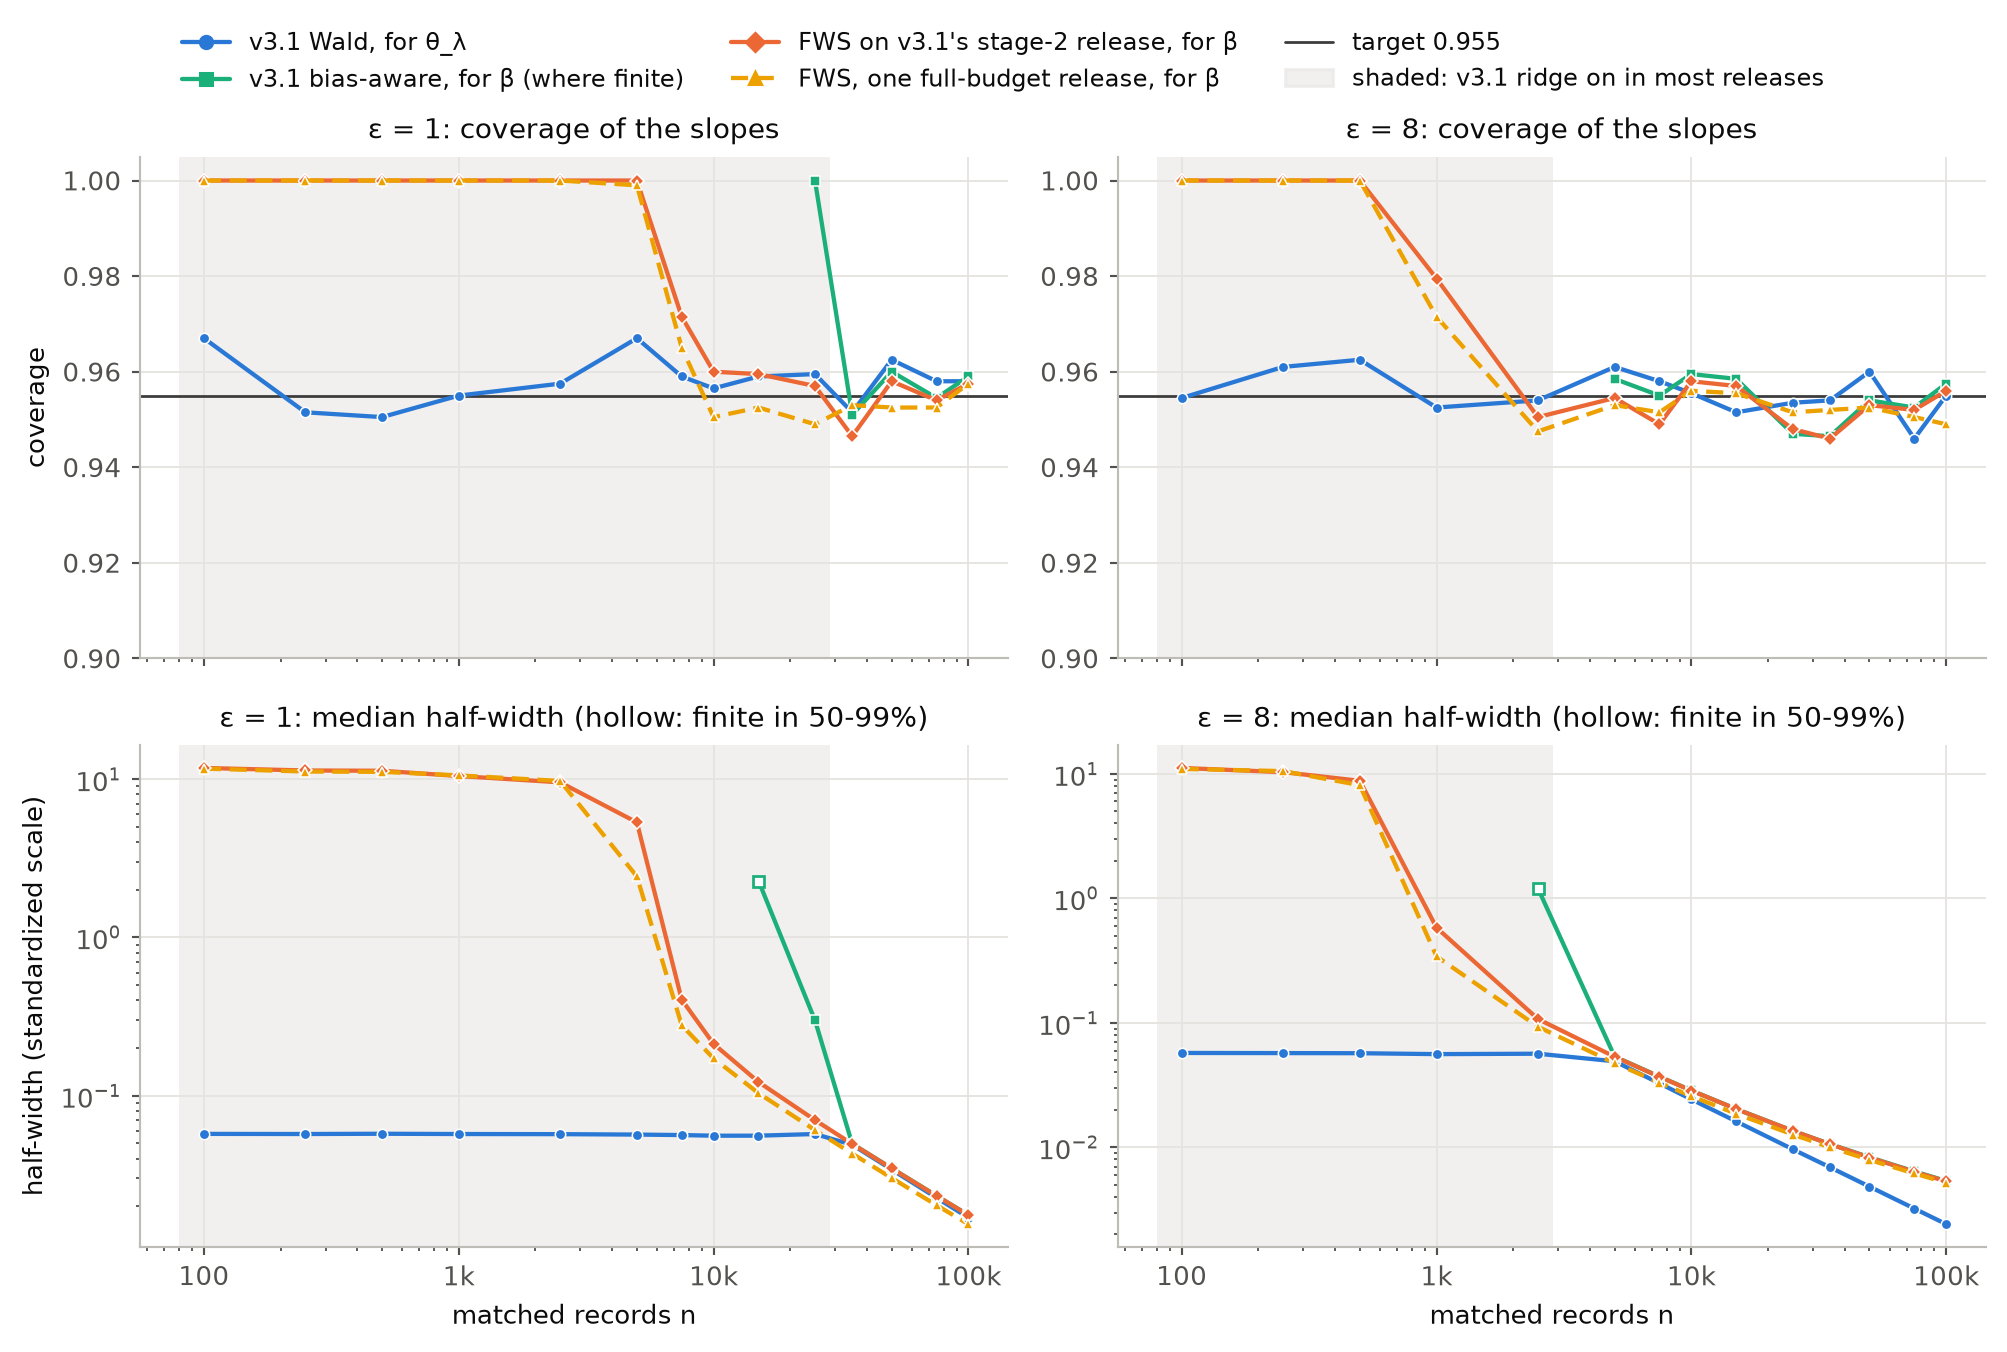
\includegraphics[width=\textwidth]{figures/fws_coverage_base.png}
  \caption{Synthetic population, setting I, $\delta = 10^{-9}$, $R^2 = 0.5$: coverage of the ten slopes (top) and median half-width (bottom, log scale) against $n$, for $\varepsilon = 1$ (left) and $8$ (right). Each interval is shown for its own target: the Wald interval for $\btheta_\lambda$, the others for $\bbeta$. The bias-aware interval is drawn only where at least half of its intervals are finite. Shaded: the stage-1 ridge is on in most releases.}
  \label{fig:fws_cov}
\end{figure}

\paragraph{Results on the synthetic population.}
\begin{itemize}
  \item \emph{The Wald interval and $\btheta_\lambda$.} The Wald interval covers $\btheta_\lambda$ $0.946$--$0.967$ in every cell, with the ridge on or off, and its half-width is $0.056$--$0.058$ while the ridge is on. FWS's interval is not centred on $\btheta_\lambda$: in the ridge-on cells where it is narrow enough to be informative it covers $\btheta_\lambda$ only $0.57$--$0.86$.
  \item \emph{Ridge off: FWS on our release is our bias-aware interval.} In the 27 cells where the ridge is off in every release, the two intervals for $\bbeta$ have the same median half-width to within $1\%$ ($0.0176$ against $0.0176$ at $n = 10^5$, $\varepsilon = 1$; $0.0053$ against $0.0054$ at $\varepsilon = 8$) and cover $0.943$--$0.958$ (FWS) and $0.946$--$0.962$ (bias-aware). With $\lambda = 0$ both add the same two variances, the mechanism's and the sampling variance, to the same estimate; one by a percentile bootstrap and the other by a Wald formula. FWS with one release covers $0.947$--$0.961$ and is $3$--$13\%$ narrower ($0.0154$ at $n = 10^5$, $\varepsilon = 1$), because it does not spend a quarter of the budget on stage~1; the difference shrinks as the sampling variance takes over ($2.6\%$ at $n = 10^5$, $\varepsilon = 8$). All three are wider than the Wald interval, which has no sampling term: read as an interval for $\bbeta$, the Wald interval covers only $0.62$ at $n = 10^5$, $\varepsilon = 8$.
  \item \emph{Ridge on: FWS is finite where the bias-aware interval is not.} While the private bound $\hat L$ is zero the bias-aware interval is unbounded: in every release at $n \le 10$k for $\varepsilon = 1$ and at $n \le 1$k for $\varepsilon = 8$. FWS uses no ridge and stays finite, and it covers $\bbeta$ in all 41 ridge-on cells ($0.951$--$1.000$). It is informative only once $\lambda_{\min}(\bG)$ is large against the noise. At $\varepsilon = 1$ its median half-width is $9.5$--$11.8$ for $n \le 2.5$k (where $\hat Q$ had to be projected in $93$--$100\%$ of releases), $5.3$ at $5$k, $0.40$ at $7.5$k, $0.21$ at $10$k, $0.12$ at $15$k and $0.070$ at $25$k ($n_{\mathrm{off}} = 27$k). At $\varepsilon = 8$ it is $8.8$--$11.1$ for $n \le 500$, $0.58$ at $1$k and $0.11$ at $2.5$k ($n_{\mathrm{off}} = 3.9$k). The change sits where $\vartheta_0 = \lambda_{\min}(\bG)/(2\sigma_2\sqrt p)$ passes $1$, near $6.4$k records at $\varepsilon = 1$ and $0.9$k at $\varepsilon = 8$. Between there and $n_{\mathrm{off}}$, FWS gives a valid finite interval for $\bbeta$ while ours is unbounded or, where $\hat L > 0$, wider (median $2.3$ at $15$k and $0.30$ at $25$k for $\varepsilon = 1$, finite ones only).
  \item \emph{FWS with one release} behaves like FWS on our release, with half-widths $13$--$41\%$ smaller in the ridge-on cells where both are informative ($0.28$ against $0.40$ at $7.5$k, $0.061$ against $0.070$ at $25$k for $\varepsilon = 1$), and coverage $0.948$--$1.000$.
\end{itemize}

\paragraph{Real data.} We repeat the comparison on three of Wang's datasets with many rows (3droad, protein and bike), with block normalization and the reference rows of fold 0 as in Section~\ref{sec:eval:adassp}. The rows outside the reference set form a finite population, and the least-squares fit of the clipped $y$ on the clipped design over all of them is the reference coefficient $\bbeta$. Cohorts of $n$ rows are drawn from it without replacement, 200 per $n$, and on each the release, the intervals and both FWS versions are computed as above ($\delta = 10^{-9}$). A cohort is at most a sixth of the population, so the finite-population correction, which makes every interval for $\bbeta$ slightly conservative, is at most $17\%$ of the sampling variance. We also ran elevators but leave it out here: its block-normalized design is nearly singular, with a population coefficient of $5.4 \times 10^4$, so its least-squares fit is not a meaningful reference. Table~\ref{tab:fws_real} gives the results.

\begin{table}[t]
  \centering
  \small
  \caption{Real data, block normalization, setting I, $\delta = 10^{-9}$, 200 cohorts per $n$ drawn from the rows outside the reference set: coverage of the slopes and, in brackets, median half-width. $\bbeta$: least-squares fit on all those rows (3droad $391{,}387$, protein $41{,}157$, bike $15{,}641$). Target $0.955$.}
  \label{tab:fws_real}
  \footnotesize
  \setlength{\tabcolsep}{3pt}
  \begin{tabular}{@{}lrrccccc@{}}
    \toprule
    & & & & \multicolumn{2}{c}{v3.1} & \multicolumn{2}{c}{FWS} \\
    \cmidrule(lr){5-6} \cmidrule(l){7-8}
    & & & & Wald & bias-aware & stage-2 & one \\
    dataset & $\varepsilon$ & $n$ & ridge & for $\btheta_\lambda$ & for $\bbeta$ & release, $\bbeta$ & release, $\bbeta$ \\
    \midrule
    3droad & 1 & 1{,}000 & 1.00 & $0.960$ ($0.148$) & $1.000$ ($2.17$) & $0.987$ ($0.606$) & $0.968$ ($0.458$) \\
     & 1 & 5{,}000 & 0.00 & $0.938$ ($0.079$) & $0.948$ ($0.089$) & $0.948$ ($0.088$) & $0.958$ ($0.078$) \\
     & 1 & 25{,}000 & 0.00 & $0.948$ ($0.016$) & $0.952$ ($0.024$) & $0.957$ ($0.024$) & $0.968$ ($0.022$) \\
     & 8 & 1{,}000 & 0.00 & $0.953$ ($0.057$) & $0.945$ ($0.107$) & $0.950$ ($0.107$) & $0.953$ ($0.102$) \\
     & 8 & 5{,}000 & 0.00 & $0.968$ ($0.011$) & $0.970$ ($0.042$) & $0.970$ ($0.042$) & $0.968$ ($0.041$) \\
     & 8 & 25{,}000 & 0.00 & $0.945$ ($0.0022$) & $0.962$ ($0.018$) & $0.958$ ($0.018$) & $0.955$ ($0.018$) \\
    \addlinespace
    protein & 1 & 1{,}000 & 1.00 & $0.962$ ($0.089$) & unbounded & $1.000$ ($16.2$) & $1.000$ ($15.9$) \\
     & 1 & 5{,}000 & 1.00 & $0.954$ ($0.087$) & unbounded & $0.998$ ($12.4$) & $0.999$ ($11.4$) \\
     & 8 & 1{,}000 & 1.00 & $0.958$ ($0.086$) & unbounded & $0.992$ ($10.4$) & $0.992$ ($9.54$) \\
     & 8 & 5{,}000 & 1.00 & $0.948$ ($0.074$) & unbounded & $0.994$ ($2.11$) & $0.983$ ($1.00$) \\
    \addlinespace
    bike & 1 & 500 & 1.00 & $0.960$ ($0.071$) & unbounded & $1.000$ ($16.3$) & $1.000$ ($16.7$) \\
     & 1 & 2{,}000 & 1.00 & $0.953$ ($0.071$) & unbounded & $1.000$ ($28.7$) & $1.000$ ($28.0$) \\
     & 8 & 500 & 1.00 & $0.967$ ($0.071$) & unbounded & $1.000$ ($24.4$) & $1.000$ ($21.5$) \\
     & 8 & 2{,}000 & 1.00 & $0.957$ ($0.078$) & unbounded & $0.940$ ($6.00$) & $0.943$ ($5.54$) \\
    \bottomrule
  \end{tabular}
\end{table}

\begin{itemize}
  \item The Wald interval covers $\btheta_\lambda$ $0.938$--$0.978$ in every cell of the four datasets (elevators included), with the ridge on or off.
  \item On 3droad ($p = 4$) the ridge is off in 11 of the 15 cells. There FWS on our release and the bias-aware interval coincide again (for example half-widths $0.088$ and $0.089$ at $n = 5$k, $\varepsilon = 1$), and both cover the population coefficient $0.945$--$0.970$, although the real errors need not be homoskedastic. In the four ridge-on cells $\hat L$ is often positive and the bias-aware interval is finite but wider than FWS's ($2.17$ against $0.61$ at $n = 1$k, $\varepsilon = 1$).
  \item On protein and bike the ridge is on in every cell ($n_{\mathrm{off}}$ is $555$k on protein at $\varepsilon = 1$, Section~\ref{sec:stats:noff}), $\hat L = 0$, and the bias-aware interval is unbounded. FWS is finite but not informative: its median half-width is $2.1$--$29$ on coefficients whose population values lie within $\pm 2$, because $\lambda_{\min}(\bG)$ is far below the noise ($\vartheta_0 \ll 1$); $\hat Q$ had to be projected in every bike release and in most protein releases at $\varepsilon \le 2$. It covers $0.93$--$1.00$; the two cells below target are protein at $n = 2.5$k and bike at $n = 2$k, both at $\varepsilon = 8$ ($0.929$ and $0.940$).
\end{itemize}

\paragraph{Why the estimands matter.} The Wald interval is narrow because $\btheta_\lambda$ is a fixed function of the matched records: it answers what the protocol would have output without the privacy noise. FWS and the bias-aware interval answer a different question, what the coefficient of the working model is, and must add the sampling variance; with the ridge off they are the same interval. They differ in how they handle a poorly conditioned design. The bias-aware interval keeps the ridge and pays for its bias with a bound on $\|\bbeta\|$, which is infinite while $\hat L = 0$. FWS drops the ridge and lets the bootstrap measure the instability of $\hat\bG_2^{-1}$, which costs variance but no bound. Once $\vartheta_0 \gtrsim 1$ that variance is moderate, and FWS is the better interval for $\bbeta$; below it, neither gives a useful interval for $\bbeta$, and only $\btheta_\lambda$ has one.

\tocheck{Consider reporting, while the ridge is on, an FWS-type percentile interval for beta from the unregularized stage-2 solve, offered only when lambda-min of G-hat-2 is at least 2 sigma-2 sqrt(p) (the gate with lambda = 0). On the synthetic population it covers where the bias-aware interval is unbounded (from about theta-0 = 1, roughly 0.25 n-off). Its validity rests on the bootstrap; it is not proved for our noise structure, and its gate would use the same release.}

\tocheck{FWS releases s-squared through its own mechanism; here it is the plug-in from the released y'y, which is biased by the noise at order sigma-2 squared, without our bootstrap correction. Check whether the correction changes FWS's coverage in the ridge-on cells.}
%NEW-END
%B-END B02

%B-BEGIN B03 Section 13.7, end of the setup: pointer to the two further baselines
%AFTER| Methods are compared by paired tests over folds (95\% CI of the mean difference of absolute test MSE, $t$ with 9 degrees of freedom).
%NEW-BEGIN
Section~\ref{sec:eval:baselines} adds two more baselines on the same folds and rows: vertical full-record SSP, which noises $\Rp$'s block too, and TukeyEM, which needs no bounds.
%NEW-END
%B-END B03

%B-BEGIN B04 New subsection after Section 13.7 (AdaSSP): full-record SSP (baseline 1) and TukeyEM (baseline 3)
%AFTER| confirm against the statement in Wang (2018) before citing it.}
%NEW-BEGIN
\subsection{Two further baselines: full-record SSP and TukeyEM}
\label{sec:eval:baselines}

Two more baselines run on the folds, reference rows and matched rows of Section~\ref{sec:eval:adassp}, at $\delta = 10^{-6}$ with 50 noise draws per fold and $\varepsilon \in \{0.5, 1, 2, 4, 8\}$, and are reported in the same two ways. They answer two questions that AdaSSP does not: what keeping $\Rp$'s block exact buys, and what the clipping bounds and the per-party preprocessing cost. They differ in what they need.
\begin{itemize}[noitemsep]
  \item \emph{Full-record SSP} could run in the vertical setting: it needs a secure aggregation of the whole Gram matrix, as in the protocols below, and output noise. With block normalization it is implementable; with joint normalization it is idealized, like arm (c).
  \item \emph{TukeyEM} needs the joined table: each of its least-squares fits uses whole rows. It is an idealized central baseline, like AdaSSP.
  \item The FWS intervals of Section~\ref{sec:eval:fws} post-process our own release, so they could run in the vertical setting.
\end{itemize}

\paragraph{Full-record SSP.} Karr et al.~\cite{karr2009privacy}, Hall et al.~\cite{hall2011secure} and Gasc\'on et al.~\cite{gascon2017privacy} compute the whole Gram matrix securely, $\bA$ included. Adding noise to every released entry gives the natural competitor that combines secure regression with output privacy. We keep everything else of v3.1: the two releases with the split $f_1$, the tight zCDP conversion with the same slack, the stage-1 rule, the gate, and settings I and P. The releases now also contain $\triu\bA$ (every entry but the constant $n$), and the adjacency replaces a whole record $(\bx_R, \bx_O, y)$. Two things change. The sensitivity is that of Proposition~\ref{prop:sens_full}. The exact radius is the quantile of $\lambda_{\max}$ of a unit noise matrix without the zero block on $\bA$, computed by the rule of Section~\ref{sec:stats:stage1}: at $p = 11$, $q_{0.9975} = 7.87$ instead of $7.42$ (setting I) and $q_{0.25} = 4.87$ instead of $4.44$ (setting P). Each full-record release adds noise on $\bA$, from a separate stream, to the same unit noise on the $\Op$-dependent entries as the v3.1 release it is compared with, so the comparison is paired draw for draw. The v3.1 arms recomputed on these streams reproduce the published fold values to $10^{-14}$. The question is therefore only what the exact $\bA$ buys.

\begin{proposition}[Sensitivity of the full-record release]
\label{prop:sens_full}
Let a record be $(\bxd, \bx_O, y)$ with $\bxd = (1, \mathbf u)$, $\|\bxd\| \le B_R$, $\|\bx_O\| \le B_O$ and $|y| \le B_y$, and let the release be the upper triangle of $\sum_i \mathbf w_i\mathbf w_i^\top$ with $\mathbf w_i = (\bxd_i, \bx_{O,i}, y_i)$, without its constant entry $n$, every entry with the same noise. For the blocks $k \in \{\mathbf u, \bx_O, y\}$ of a record and of its replacement write $n_k$ and $n'_k$ for their squared norms and $g_k$ for their inner product. Then the replace-one $\ell_2$ sensitivity is
\begin{equation}
  \Delta_{\mathrm{full}}^2 = \sup\Bigl[\sum_k (n_k + n'_k - 2g_k) + \sum_k (n_k^2 + n_k'^2 - 2g_k^2) + \sum_{k < l} (n_k n_l + n'_k n'_l - 2g_k g_l)\Bigr],
  \label{eq:sens_full}
\end{equation}
over the norms allowed by the bounds and $|g_k| \le \sqrt{n_k n'_k}$, with $|g_k| = \sqrt{n_k n'_k}$ for a block of dimension one ($y$ among them). For a block of dimension at least two the supremum is attained with both norms at the bound. Without an intercept the first sum is dropped; without $\by^\top\by$ (separate mode) the term $(n_y - n'_y)^2$ is dropped; for stage~1 every term with $y$ is dropped.
\end{proposition}

\begin{proof}[Proof sketch]
The first sum is the change of the first moments (the intercept row), the others that of $\triu(\mathbf w\mathbf w^\top - \mathbf w'\mathbf w'^\top)$ block by block. For each diagonal block $\|\triu \bS\|^2 \le \|\bS\|_F^2$, which gives the bound. In two coordinates, for any norms and inner product, the two vectors can be chosen so that $\mathbf x\mathbf x^\top - \mathbf x'\mathbf x'^\top$ is diagonal, so the bound is attained for blocks of dimension at least two. The bracket is a concave quadratic in the $g_k$, every other coefficient is nonnegative, and the admissible set of $g_k$ grows with the norms, so its maximum is nondecreasing in $n_k$ and $n'_k$. What remains, $(y, y')$ and the norms of one-dimensional blocks, is maximized on a dense grid and refined by local search, with the result rounded up by a relative $10^{-12}$ as for Proposition~\ref{prop:sens}. With $\Rp$'s row held fixed the same computation reproduces Proposition~\ref{prop:sens} to $10^{-12}$, and a direct maximization over vectors with $d_R, d_O \in \{1, 2, 3\}$ from many starting points never exceeds~\eqref{eq:sens_full} and attains it.
\end{proof}

Without an intercept and at unit bounds (arm (c), $d_R, d_O \ge 2$), $\Delta_{\mathrm{full}}^2 = 32/3$ (at $\cos\angle(\mathbf u, \mathbf u') = \cos\angle(\bx_O, \bx'_O) = 1/3$ and $y' = -y$) against $\Delta^2 = 10$, and $\Delta_{G,\mathrm{full}}^2 = 6$ against $\Delta_G^2 = 4.5$. On the simulation population (standardized, $B_R = 5.59$ with the intercept, $B_O = 6.24$, $B_y = 2.89$), $\Delta$ rises from $86.2$ to $92.7$ ($+7.5\%$) and $\Delta_G$ from $77.2$ to $85.8$ ($+11\%$). Under block normalization the sensitivity of the stage-2 release without $\by^\top\by$, which sets $\sigma_2$ there because $\by^\top\by$ is released separately, does not change at all ($10.00$ at $B_y = 2.89$), and $\Delta_G$ rises from $2.83$ to $3.27$ ($+15\%$). On the 29 datasets (fold 0, $\varepsilon = 1$), $\sigma_1$ rises by $12$--$16\%$ and $\sigma_2$ by $0$--$7\%$ under block normalization, and by $0$--$16\%$ and $0$--$3\%$ under joint normalization.

\begin{table}[t]
  \centering
  \small
  \caption{Full-record SSP against v3.1 on the simulation population ($\delta = 10^{-9}$, $R^2 = 0.5$, the cohorts and unit noise of Section~\ref{sec:eval:sim}): matched records at which the stage-1 ridge switches off ($n_{\mathrm{off}}$ of~\eqref{eq:noff} with the full-record noise and radius), at which test MSE comes within $10\%$ of non-private least squares, and at which the median slope RMSE reaches twice the OLS floor. Each cell: v3.1 / full-record. ``$>$100k'': not reached.}
  \label{tab:full_sim}
  \setlength{\tabcolsep}{3pt}
  \begin{tabular}{@{}rcccccc@{}}
    \toprule
    & \multicolumn{3}{c}{setting I} & \multicolumn{3}{c}{setting P} \\
    \cmidrule(lr){2-4} \cmidrule(l){5-7}
    $\varepsilon$ & $n_{\mathrm{off}}$ & prediction $\le 1.1$ & slopes $\le 2\times$ & $n_{\mathrm{off}}$ & prediction $\le 1.1$ & slopes $\le 2\times$ \\
    \midrule
    0.5 & 52.5k / 58.7k & 38.1k / 42.8k & $>$100k / $>$100k & 31.5k / 35.7k & 26.5k / 30.5k & $>$100k / $>$100k \\
    1 & 27.0k / 30.2k & 20.1k / 22.1k & $>$100k / $>$100k & 16.2k / 18.4k & 13.7k / 15.8k & $>$100k / $>$100k \\
    2 & 13.9k / 15.6k & 10.0k / 11.6k & 88.2k / $>$100k & 8.4k / 9.5k & 7.1k / 8.2k & 88.2k / $>$100k \\
    4 & 7.3k / 8.1k & 5.3k / 6.0k & 26.6k / 31.6k & 4.4k / 4.9k & 4.0k / 4.3k & 26.6k / 31.6k \\
    8 & 3.9k / 4.3k & 2.9k / 3.4k & 8.0k / 9.4k & 2.3k / 2.6k & 2.1k / 2.2k & 8.0k / 9.4k \\
    \midrule
    \multicolumn{7}{@{}l}{block-normalized population: prediction $\le 1.1$} \\
    0.5 & & 14.7k / 15.4k & & & 9.4k / 9.8k & \\
    1 & & 7.5k / 7.9k & & & 4.8k / 5.1k & \\
    2 & & 4.0k / 4.1k & & & 2.5k / 2.7k & \\
    4 & & 2.1k / 2.1k & & & 1.5k / 1.6k & \\
    8 & & 1.1k / 1.2k & & & 729 / 767 & \\
    \bottomrule
  \end{tabular}
\end{table}

\begin{figure}[t]
  \centering
  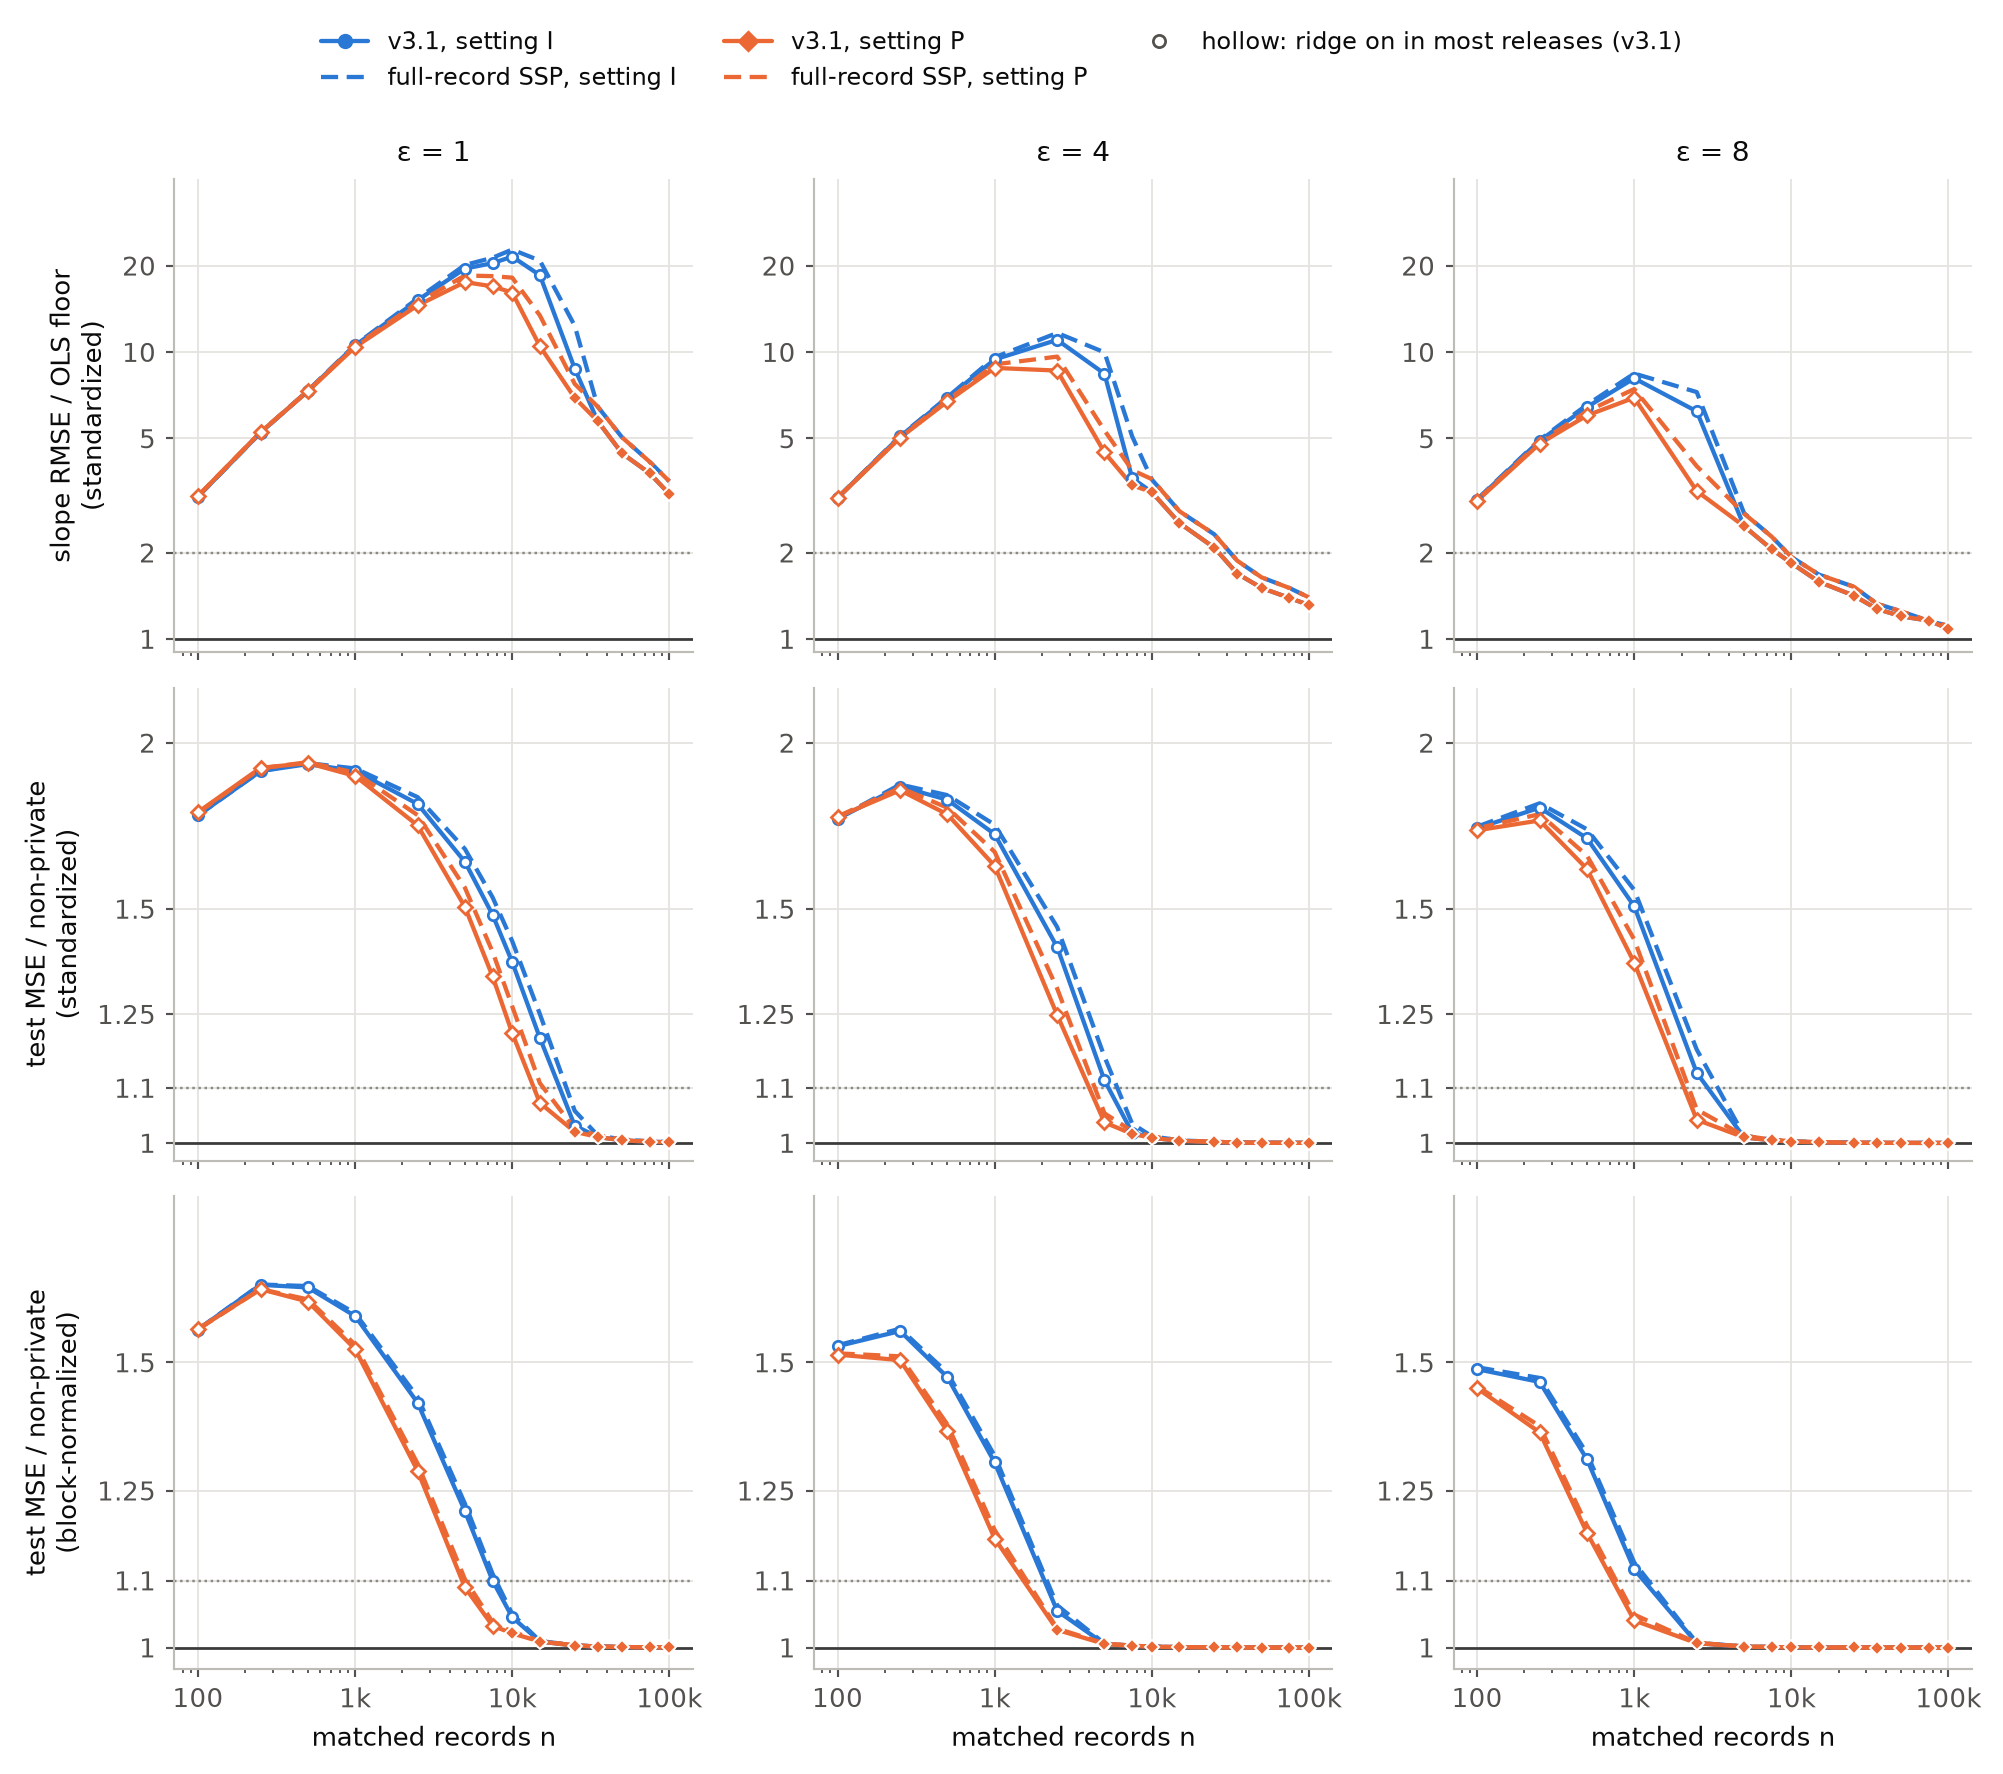
\includegraphics[width=\textwidth]{figures/fullrecord_sim_base.png}
  \caption{Full-record SSP (dashed) against v3.1 (solid) on the simulation population, $\delta = 10^{-9}$, $R^2 = 0.5$; blue: setting I, orange: setting P; columns $\varepsilon = 1$, $4$, $8$. Top: median slope RMSE divided by that of non-private least squares (standardized population). Middle and bottom: population test MSE divided by that of non-private least squares on the same cohort, for the standardized and the block-normalized population. Hollow markers: the v3.1 ridge is on in most releases.}
  \label{fig:full_sim}
\end{figure}

\paragraph{Results for full-record SSP.}
\begin{itemize}
  \item \emph{Synthetic population, standardized} (Table~\ref{tab:full_sim}, Figure~\ref{fig:full_sim}). Noising $\bA$ moves every threshold up. The ridge switches off $12\%$ later under setting I and $13\%$ later under P ($30.2$k against $27.0$k records at $\varepsilon = 1$ under I). Prediction within $10\%$ of non-private needs $7$--$16\%$ more records ($22.1$k against $20.1$k under I and $15.8$k against $13.7$k under P at $\varepsilon = 1$). Twice the OLS floor on the slopes needs $17$--$18\%$ more ($31.6$k against $26.6$k at $\varepsilon = 4$, $9.4$k against $8.0$k at $\varepsilon = 8$), and at $\varepsilon = 2$ it is not reached by $10^5$ records ($88$k for v3.1). Once the ridge is off the slopes stay less accurate: at $n = 10^5$ their median RMSE is $3.54$ against $3.20$ times the floor at $\varepsilon = 1$, and $1.40$ against $1.31$ at $\varepsilon = 4$.
  \item \emph{Synthetic population, block-normalized.} Here $\sigma_2$ is unchanged and only stage~1 and the noise on $\bA$ cost. Prediction within $10\%$ needs $3$--$7\%$ more records.
  \item \emph{The 29 datasets} (Table~\ref{tab:full_verdicts}, Figure~\ref{fig:full_real}). Full-record SSP has significantly higher test MSE than v3.1 on most datasets and lower on few, but the gap is small. Under block normalization and setting I it is higher on $21$--$24$ of $29$ datasets and lower on at most $2$, at every $\varepsilon$, with a median gap of $+0.4\%$ to $+1.0\%$; under setting P, higher on $19$--$23$ and lower on at most $2$, by $+0.6\%$ to $+1.2\%$. The largest gaps are on energy and sml ($+5.1\%$ and $+4.1\%$ under I at $\varepsilon = 1$, $+7.3\%$ and $+6.3\%$ under P). Under joint normalization the median gap is $+1.0\%$ to $+1.7\%$; full-record SSP is lower on $7$ datasets at $\varepsilon = 0.5$ and $5$ at $\varepsilon = 1$ under setting I. Six of the seven have little linear signal (non-private test MSE within $25\%$ of that of predicting the mean: fertility, forest, pendulum, pumadyn32nm, solar and tamielectric), where its larger ridge shrinks a noisy estimate further; the seventh is concreteslump ($103$ rows). Its median ridge is $8$--$10\%$ larger than v3.1's under block normalization and $14$--$17\%$ under joint normalization. Its gate refused $0.14\%$ of releases on average under block normalization and setting P at $\varepsilon = 1$ (at most $2.4\%$, solar).
  \item \emph{Against AdaSSP} the verdicts do not change: under block normalization and setting I full-record SSP is worse than AdaSSP (published) on $20$ of $29$ datasets at $\varepsilon = 1$ with a median gap of $+26\%$, against $+25\%$ for v3.1.
\end{itemize}
Keeping $\Rp$'s block exact therefore buys about $1\%$ of test MSE on real data with per-party preprocessing, consistently but little, and $7$--$18\%$ of the records needed on standardized synthetic data, where $\Rp$'s bound is large ($B_R = 5.59$). The gain grows with $\Rp$'s share of the sensitivity: under block normalization $B_y$ dominates $\Delta$, so the exact $\bA$ saves only the noise on $\bA$ itself and part of $\Delta_G$. Its other benefits are that no budget and no circuit work are spent on statistics that $\Rp$ already holds, and that $\Rp$ can use the exact $\bA$ for diagnostics that cost no budget (Section~\ref{sec:stats:noff}).

\begin{table}[t]
  \centering
  \small
  \caption{Full-record SSP on the 29 datasets, $\delta = 10^{-6}$: number of datasets on which it has significantly lower / higher absolute test MSE than the arm it is compared with (95\% CI over folds, $t$ with 9 degrees of freedom), and in brackets the median over datasets of the ratio of their test MSE, minus one, in percent. First four rows: against v3.1 with the same preprocessing and setting. The verdicts on the ratio to the own non-private fit differ by at most one dataset.}
  \label{tab:full_verdicts}
  \footnotesize
  \setlength{\tabcolsep}{3.5pt}
  \begin{tabular}{@{}lccccc@{}}
    \toprule
    Full-record SSP & $\varepsilon = 0.5$ & $\varepsilon = 1$ & $\varepsilon = 2$ & $\varepsilon = 4$ & $\varepsilon = 8$ \\
    \midrule
    (d) block norm, I & 1/21 ($+0.4$) & 1/23 ($+0.7$) & 2/23 ($+1.0$) & 1/24 ($+0.8$) & 0/24 ($+0.6$) \\
    (d) block norm, P & 2/19 ($+0.6$) & 1/20 ($+0.9$) & 2/22 ($+1.2$) & 0/23 ($+0.8$) & 0/23 ($+0.7$) \\
    (c) joint norm, I & 7/21 ($+1.0$) & 5/21 ($+1.6$) & 3/22 ($+1.7$) & 2/23 ($+1.1$) & 0/24 ($+1.1$) \\
    (c) joint norm, P & 7/20 ($+1.3$) & 5/21 ($+1.5$) & 5/22 ($+1.7$) & 3/21 ($+1.0$) & 1/23 ($+1.0$) \\
    (d), P vs v3.1 (d), I & 18/2 ($-2.7$) & 22/1 ($-3.8$) & 24/1 ($-5.5$) & 24/1 ($-3.8$) & 23/0 ($-3.7$) \\
    (d), I vs (a) AdaSSP, published & 6/19 ($+15.6$) & 5/20 ($+25.9$) & 4/21 ($+20.2$) & 3/22 ($+13.8$) & 1/21 ($+11.2$) \\
    (d), P vs (a) & 6/19 ($+10.3$) & 5/20 ($+15.4$) & 5/19 ($+11.7$) & 2/20 ($+9.0$) & 3/16 ($+5.3$) \\
    (c), P vs (b) AdaSSP, matched & 7/15 ($+1.3$) & 6/18 ($+6.8$) & 6/19 ($+4.8$) & 4/19 ($+3.3$) & 1/20 ($+4.6$) \\
    \bottomrule
  \end{tabular}
\end{table}

\begin{figure}[t]
  \centering
  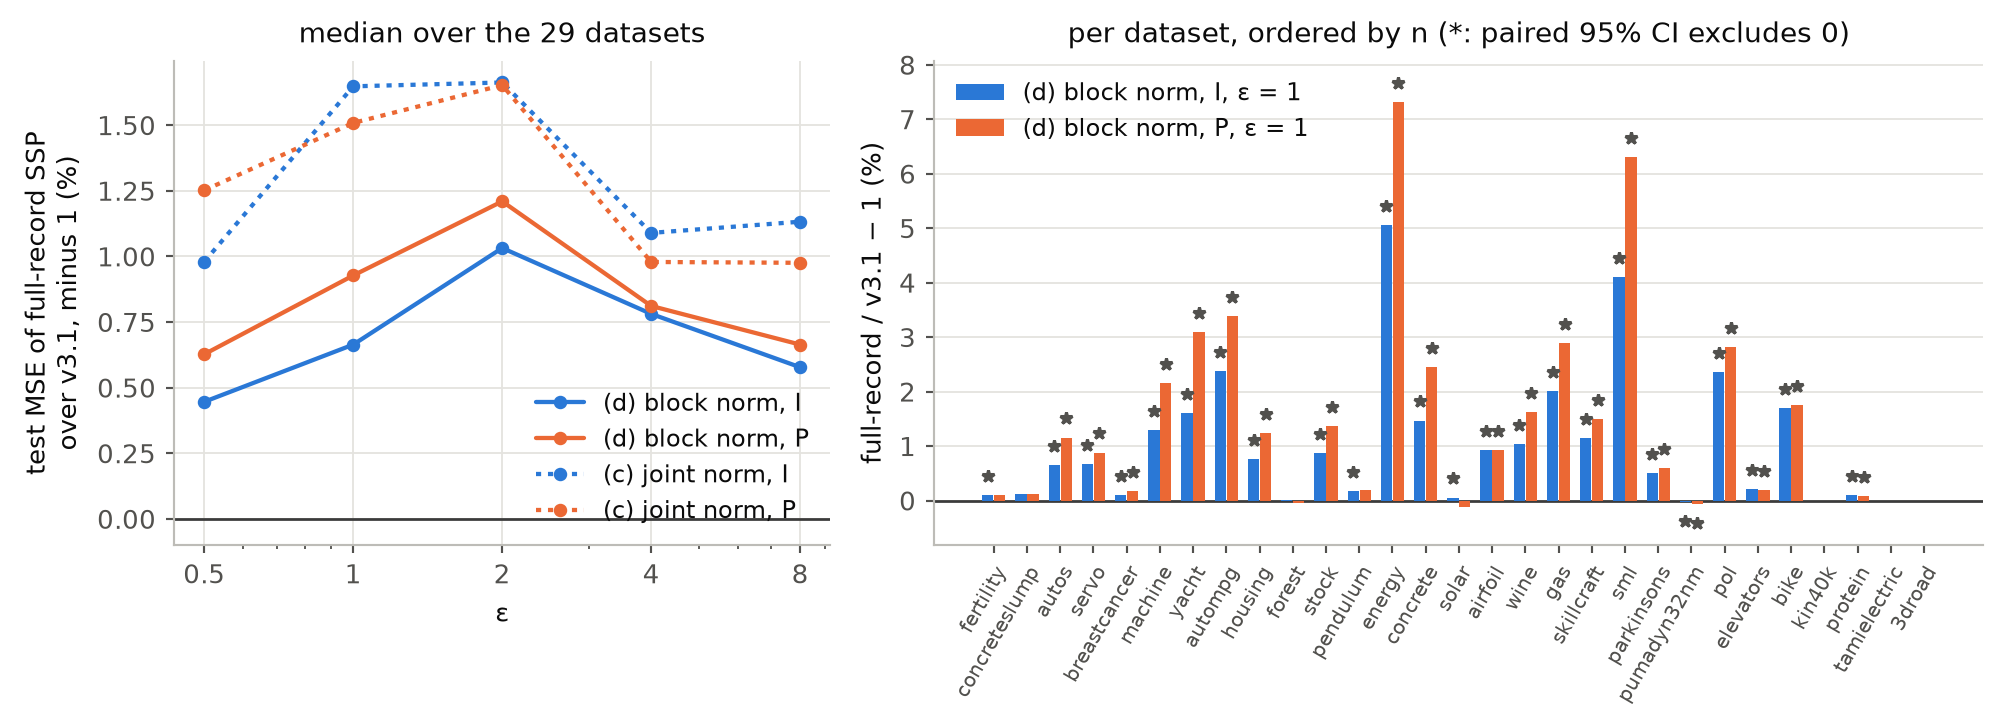
\includegraphics[width=\textwidth]{figures/fullrecord_real_base.png}
  \caption{Full-record SSP against v3.1 on the 29 datasets, $\delta = 10^{-6}$. Left: median over datasets of the absolute test MSE of full-record SSP divided by that of v3.1 with the same preprocessing and setting, minus one, against $\varepsilon$. Right: the same per dataset at $\varepsilon = 1$, block normalization; a star marks a paired 95\% CI over folds that excludes zero.}
  \label{fig:full_real}
\end{figure}
\paragraph{TukeyEM.} Amin et al.~\cite{amin2023easy} split the rows at random into $m$ disjoint groups, fit least squares on each, and release a point of high approximate Tukey depth among the $m$ fits. A propose-test-release (PTR) step first checks, with half the budget, that the regions of high depth are stable; if the check fails, nothing is released, which we score as $\btheta = 0$, as a refused release of v3.1. The exponential mechanism on depth uses the other half. A record changes one fit, so the guarantee is $(\varepsilon, \delta)$-DP for a change of one whole record, at the nominal $(\varepsilon, \delta) = (\varepsilon, 10^{-6})$ and with no zCDP conversion. TukeyEM needs no bound on the features or the labels, so it runs on the z-scored features (reference-set constants, with an intercept column) and the standardized $y$, without clipping; its own non-private fit is the ridge fit on that design. We reimplemented it from the reference code (\texttt{dp\_regression/tukey.py} of \texttt{github.com/google-research/google-research}, commit \texttt{ba728e2}). Replaying the reference code's random numbers, the two give the same fits, PTR distances and outputs in 60 of 60 trials. We changed three details of the reference code:
\begin{itemize}[noitemsep]
  \item the Laplace noise of the PTR test has scale $1/(\varepsilon/2)$, which its threshold $\ln(1/(2\delta))/(\varepsilon/2)$ requires, instead of $\varepsilon/2$;
  \item the released point is drawn from the depth level that the exponential mechanism chose, not from the next deeper one;
  \item an empty set of depths in the PTR check counts as passing instead of raising an error.
\end{itemize}
On the reference code's own example ($n = 22{,}000$, $d = 10$) the first two leave the pass rates unchanged and raise the median error of the released model by $0.1$--$5\%$. The number of groups trades the PTR test against the accuracy of each fit. We fixed it in advance to groups of $2p$ rows, $m = \lfloor n/(2p) \rfloor$, close to the reference example ($m = 1{,}000$ to $2{,}000$ at $n = 22{,}000$, $p = 11$). We also ran $m = \lfloor n/(kp) \rfloor$ for $k \in \{1.5, 3, 5, 10, 25\}$; choosing the best $k$ per dataset and $\varepsilon$ on the test folds, an optimistic oracle, changes the counts against v3.1 below by at most one dataset.

\paragraph{Where TukeyEM fails.} The PTR distance is a lower bound on the number of fits that would have to change to make the release unsafe. It cannot exceed $t - 1$ with $t = \lfloor\lfloor m/2\rfloor/2\rfloor$, and the test passes only if the distance plus Laplace noise exceeds $\ln(1/(2\delta))/(\varepsilon/2)$, which is $26.2$ at $\varepsilon = 1$ and $3.3$ at $\varepsilon = 8$ for $\delta = 10^{-6}$. So TukeyEM needs about $m \ge 110$ groups at $\varepsilon = 1$ and $m \ge 20$ at $\varepsilon = 8$, that is $n \ge 220p$ and $n \ge 40p$ matched rows with groups of $2p$. With our split, $21$ of the $29$ datasets have $m < 110$ and $12$ have $m < 20$. Enough groups are necessary but not sufficient: the regions of high depth are stable only if the fits agree, which fits on $2p$ rows rarely do. Table~\ref{tab:tukey} and Figure~\ref{fig:tukey} give the results.
\begin{itemize}
  \item \emph{The test fails on every dataset with fewer than about $3{,}500$ rows per coefficient, unless $\varepsilon$ is large.} At $\varepsilon \le 2$ it passes in every run on kin40k, protein, tamielectric and 3droad ($n/p \ge 3{,}556$, $m \ge 1{,}777$) and in no run on the other $25$ datasets. There its distance bound takes its smallest value, $-1$, even where $m$ would allow more (pol, elevators and bike, $m = 222$--$386$). At $\varepsilon = 8$ it also passes on pol, elevators, bike and airfoil ($98\%$), and fails on the other 21 datasets in every run.
  \item \emph{Where it passes, it is accurate on the large datasets.} Its test MSE is within $0.4\%$ of its own non-private fit on kin40k, tamielectric and 3droad, and $12\%$ ($\varepsilon = 1$) and $8\%$ ($\varepsilon = 8$) above it on protein. At $\varepsilon = 8$ it is $1.2\%$ above on bike, $6\%$ on airfoil and $15\%$ on elevators. On pol it passes at $\varepsilon = 8$ but releases a poor model: $5.3$ times its non-private test MSE and $7.4$ times that of v3.1. Its fits on groups of $54$ rows vary widely (pol's features are discrete), and the released model predicts worse than the mean ($0.983$ against $0.345$ on Wang's scale).
  \item \emph{Against v3.1.} TukeyEM has significantly higher absolute test MSE than v3.1 with block normalization under setting P on $25$ of $29$ datasets at $\varepsilon = 1$ and lower on $2$ (median gap $+26\%$), and higher on $24$ and lower on $3$ at $\varepsilon = 8$ ($+31\%$). Against setting I the counts are $25$ and $1$ ($+18\%$) and $24$ and $3$ ($+30\%$). It is lower on 3droad, where the unclipped z-scored fit beats block normalization ($0.02649$ against $0.02689$ non-private), on pumadyn32nm, where the test fails and predicting the mean beats any fit of these noise-only data, and at $\varepsilon = 8$ on elevators, where block normalization's own non-private fit is $2.6$ times worse than the z-scored one.
\end{itemize}
TukeyEM therefore answers the question about bounds only where it passes. There, the bounds and the clipping of v3.1 cost little: on protein, kin40k and tamielectric v3.1 is as accurate or more so. Per-party block normalization can cost more than the privacy noise (elevators), and a method without bounds avoids that cost, but at the sizes of most of Wang's datasets TukeyEM releases nothing.

\begin{table}[t]
  \centering
  \small
  \caption{TukeyEM on the datasets where its PTR test passes at some $\varepsilon$ ($\delta = 10^{-6}$, $m = \lfloor n/(2p)\rfloor$ groups, 10 folds, 50 runs per fold): share of runs that pass, test MSE divided by its own non-private fit, and absolute test MSE divided by that of v3.1 with block normalization under setting P, at $\varepsilon = 1$ / $8$. On the other 21 datasets the test fails in every run at every $\varepsilon$.}
  \label{tab:tukey}
  \setlength{\tabcolsep}{4pt}
  \begin{tabular}{@{}lrrrccc@{}}
    \toprule
    Dataset & $n$ & $p$ & $m$ & PTR passes & ratio to own fit & ratio to v3.1 (d), P \\
    \midrule
    airfoil & 1{,}203 & 6 & 100 & 0.00 / 0.98 & 2.041 / 1.059 & 1.565 / 1.026 \\
    pol & 12{,}000 & 27 & 222 & 0.00 / 1.00 & 1.872 / 5.335 & 2.027 / 7.440 \\
    elevators & 13{,}280 & 19 & 349 & 0.00 / 1.00 & 4.170 / 1.147 & 1.448 / 0.420 \\
    bike & 13{,}904 & 18 & 386 & 0.00 / 1.00 & 3.721 / 1.012 & 3.264 / 1.066 \\
    kin40k & 32{,}000 & 9 & 1{,}777 & 1.00 / 1.00 & 1.004 / 1.003 & 1.007 / 1.007 \\
    protein & 36{,}584 & 10 & 1{,}829 & 1.00 / 1.00 & 1.116 / 1.083 & 1.092 / 1.074 \\
    tamielectric & 36{,}625 & 4 & 4{,}578 & 1.00 / 1.00 & 1.001 / 1.001 & 1.001 / 1.001 \\
    3droad & 347{,}900 & 4 & 43{,}487 & 1.00 / 1.00 & 1.002 / 1.002 & 0.988 / 0.988 \\
    \bottomrule
  \end{tabular}
\end{table}

\begin{figure}[t]
  \centering
  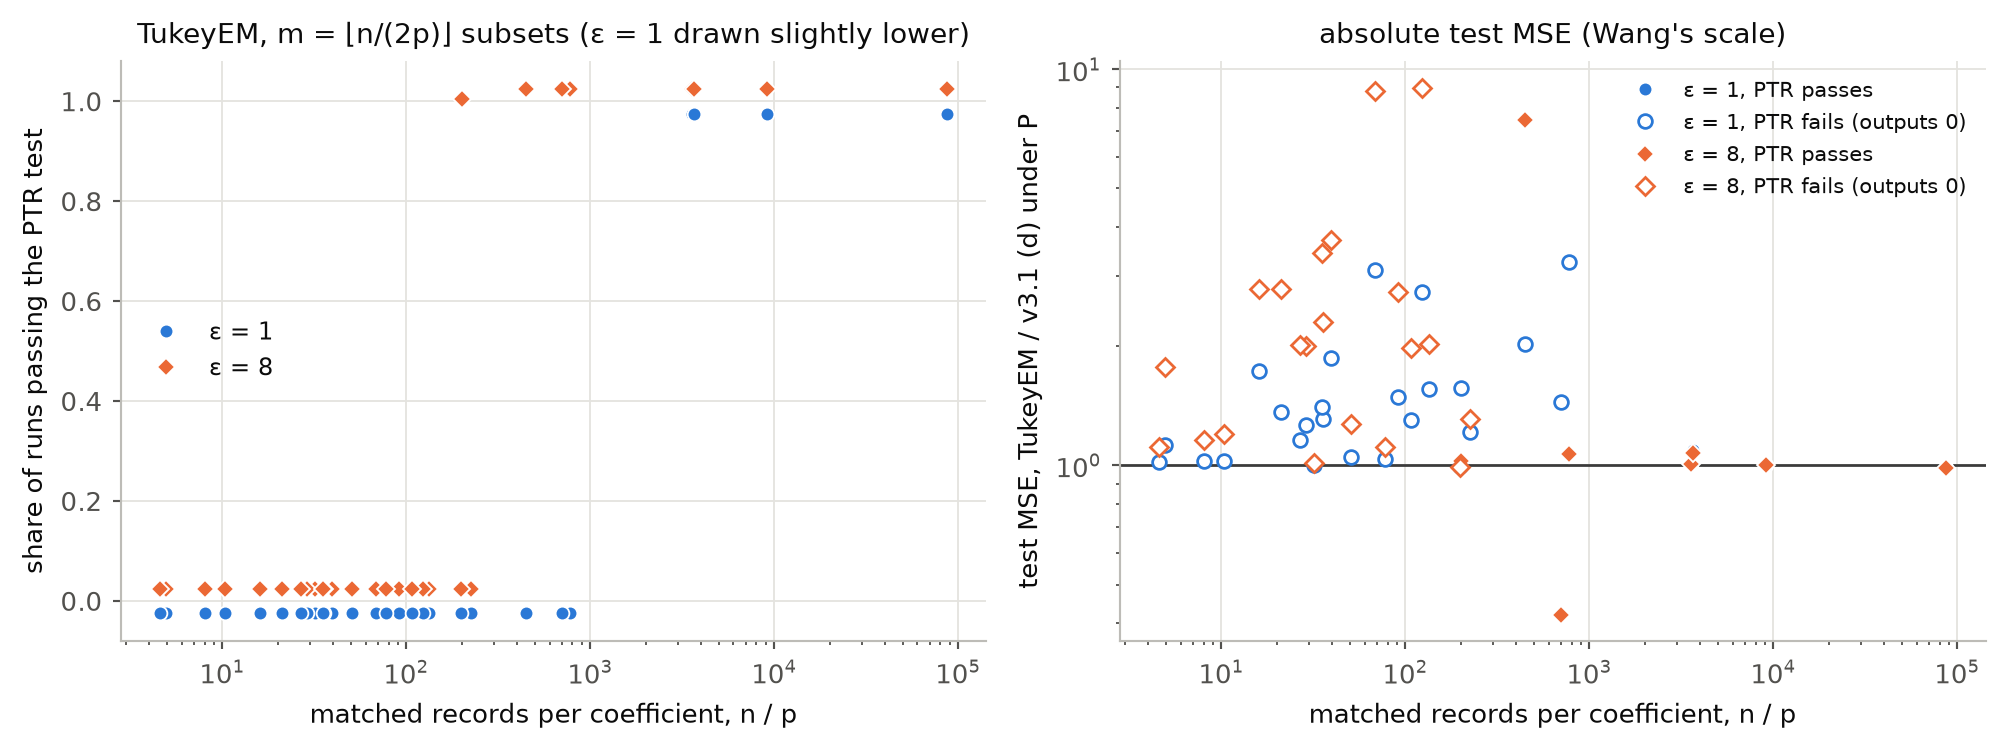
\includegraphics[width=\textwidth]{figures/tukey_base.png}
  \caption{TukeyEM on the 29 datasets, $\delta = 10^{-6}$, $m = \lfloor n/(2p)\rfloor$ groups, against matched rows per coefficient. Left: share of runs that pass the PTR test, at $\varepsilon = 1$ (circles, drawn slightly lower) and $8$ (diamonds). Right: absolute test MSE divided by that of v3.1 with block normalization under setting P; hollow: the test fails in most runs, so TukeyEM outputs $\btheta = 0$.}
  \label{fig:tukey}
\end{figure}

\tocheck{TukeyEM: the adjacency (a change of one record changes one of the m fits; the PTR distance is a Hamming distance between the sets of fits) and the PTR noise scale 2/epsilon are taken from the reference code and the PTR threshold, because the paper of Amin et al. was not accessible when this was written. Confirm both against the paper, and the choice of m against its recommendation.}

\tocheck{Full-record SSP was simulated in plaintext only. Its cryptographic cost (aggregating A under encryption as well, d-R (d-R + 1)/2 more released entries per release) is not measured, and a secure-aggregation protocol of the kind of Karr et al. or Gascon et al. would have its own cost.}

\tocheck{Full-record SSP: the sensitivity of the full-record release is computed numerically after the monotonicity reduction (a grid over y and y-prime, refined by local search). Derive closed forms, as for Proposition prop:sens, or keep the numerical computation and its checks.}
%NEW-END
%B-END B04

%B-BEGIN B05 Section 13.9 (where the utility goes): what the other baselines add
%AFTER| Per-party block normalization costs little against Wang's joint normalization, which no party can apply in the vertical setting
%NEW-BEGIN
\paragraph{What the other baselines add.} Three comparisons bound the cost of the design choices (Sections~\ref{sec:eval:fws} and~\ref{sec:eval:baselines}).
\begin{itemize}[noitemsep]
  \item \emph{The exact $\bA$ is a modest accuracy gain.} Noising $\Rp$'s block as well, with the protocol otherwise unchanged, raises test MSE by a median of $0.4$--$1.7\%$ on the 29 datasets (significantly on $19$--$24$ of them, at every $\varepsilon$, setting and preprocessing), and the records needed on the standardized synthetic population by $7$--$18\%$. The exact $\bA$ also means that no budget and no circuit work are spent on statistics that $\Rp$ already holds.
  \item \emph{Dropping the bounds does not help at these sizes.} TukeyEM, on the joined table and without bounds, fails its stability test on $25$ of $29$ datasets at $\varepsilon \le 2$ and has higher test MSE than v3.1 under setting P on $24$--$25$ of them. Where it passes, it shows that block normalization can cost more than the privacy noise (elevators), and that clipping costs little (protein, kin40k).
  \item \emph{For $\bbeta$, a bootstrap without the ridge helps where ours gives no interval.} The interval of Ferrando et al.\ on our stage-2 release equals our bias-aware interval once the ridge is off, and stays finite and covers while the ridge is on, from about $\vartheta_0 = 1$, roughly a quarter of $n_{\mathrm{off}}$ on the synthetic population. Below that, only $\btheta_\lambda$ has a useful interval.
\end{itemize}
%NEW-END
%B-END B05

%B-BEGIN B06 Table tab:settings (Section 12): narrower columns, because the two new subsections renumber 13.4-13.9 to 13.5-13.11 and the row "used in" then overflows by 9.5pt
%OLD| \setlength{\tabcolsep}{4pt}
%OLD| \begin{tabular}{@{}lllll@{}}
%NEW-BEGIN
\setlength{\tabcolsep}{2.5pt}
\begin{tabular}{@{}lllll@{}}
%NEW-END
%B-END B06
